\chapter{リフトについて}

\section{要求される仕様}
\subsection{ロボコンのルール}
今年度のロボコンのタイトルは「ロボット・ニューフロンティア」で,新大陸の開拓をテーマとしている.今回の競技フィールドを(図\ref{fig:field})に示す.新大陸では,スタート地点から運んできたプラスティック製段ボールの箱(図\ref{fig:plabox})を高く積み上げる課題が課されている.港町と島,島と新大陸までの間の海にはロボットは接地してはならない.積み上げロボットはスタート地点と島に置いてあるプラスティック製段ボールを取りに行き高台に小さい砦を積み上げる.高台の砦が完成後,新大陸に向かい丘に砦を完成させる.これを2チームでいかに高く積み上げるかを競い合う競技となっている.

\begin{figure}[htbp]
  \begin{center}
    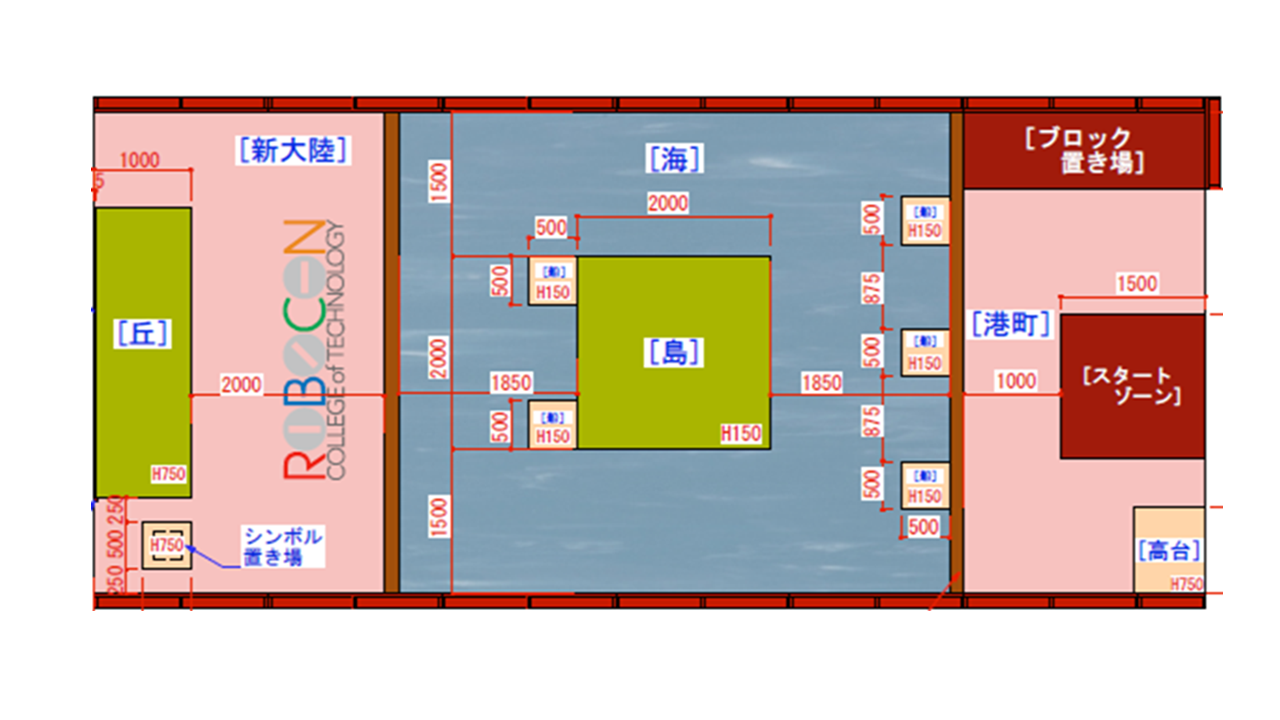
\includegraphics[width=130mm]{img/field.png}
    \end{center}
  \caption{競技フィールド}
 \label{fig:field}
\end{figure}

\subsection{我々の戦略}
プラスティック製段ボールの積み方を(図\ref{fig:tumikata})に示すように,同じ数の箱を積み上げる場合,箱の長手方向を縦向きにして積み上げる方が高く積み上げられる.よってリフトの可動高さを400[mm]になるよう設計,製作した.だが,長手方向を縦向きにすることで重心位置が高くなり,底面積が減るため落下時にバランスが崩れ,倒れる恐れがあるため注意する必要がある.


\begin{figure}[htbp]
  \begin{center}
    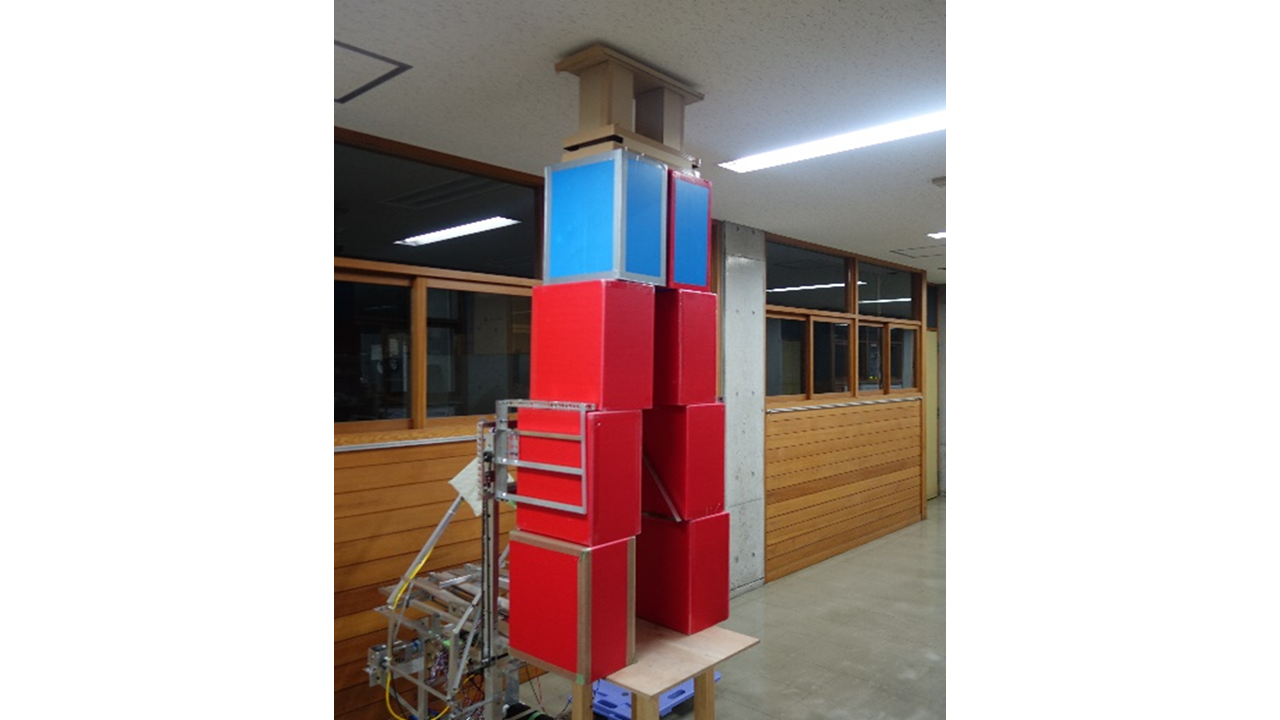
\includegraphics[width=90mm]{img/tumikata.png}
    \end{center}
  \caption{プラスティック段ボールの積み方}
 \label{fig:tumikata}
\end{figure}

\begin{figure}[htbp]
  \begin{center}
    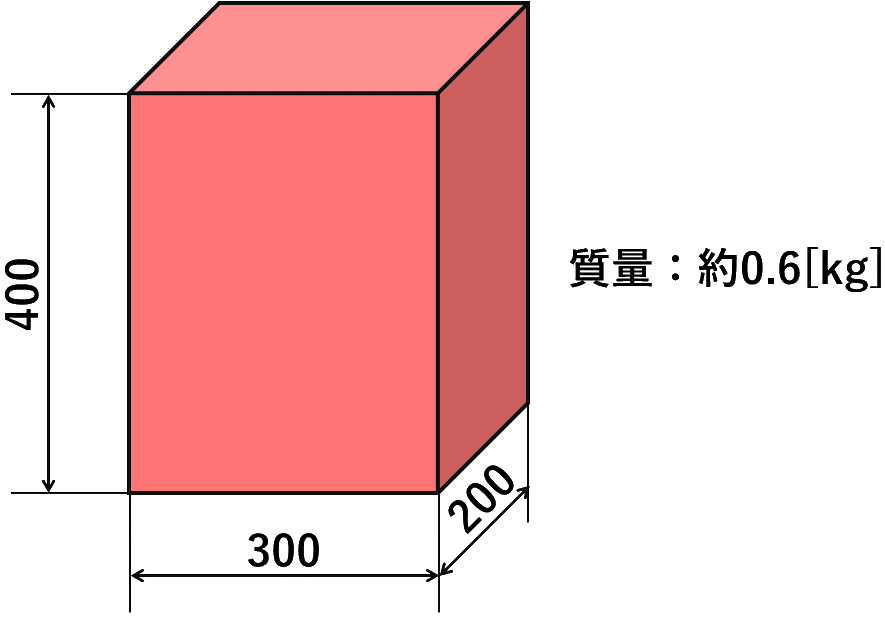
\includegraphics[width=100mm]{img/plabox.png}
    \end{center}
  \caption{プラ段の箱の仕様}
 \label{fig:plabox}
\end{figure}




\section{動作原理}
積込ロボットの前面にリフトが搭載されている(図\ref{fig:lift}).
リフト中央下部に設置されているモータによってスプロケットが回転し,チェーン駆動をする.
リフト上端と下端に設置してあるリミットセンサには通過型フォトインタラプタを使用している.リミットセンサは距離が400[mm]になるように位置が調整されているため,箱を400[mm]の高さに持ち上げることが出来る.



\begin{figure}[htbp]
  \begin{center}
    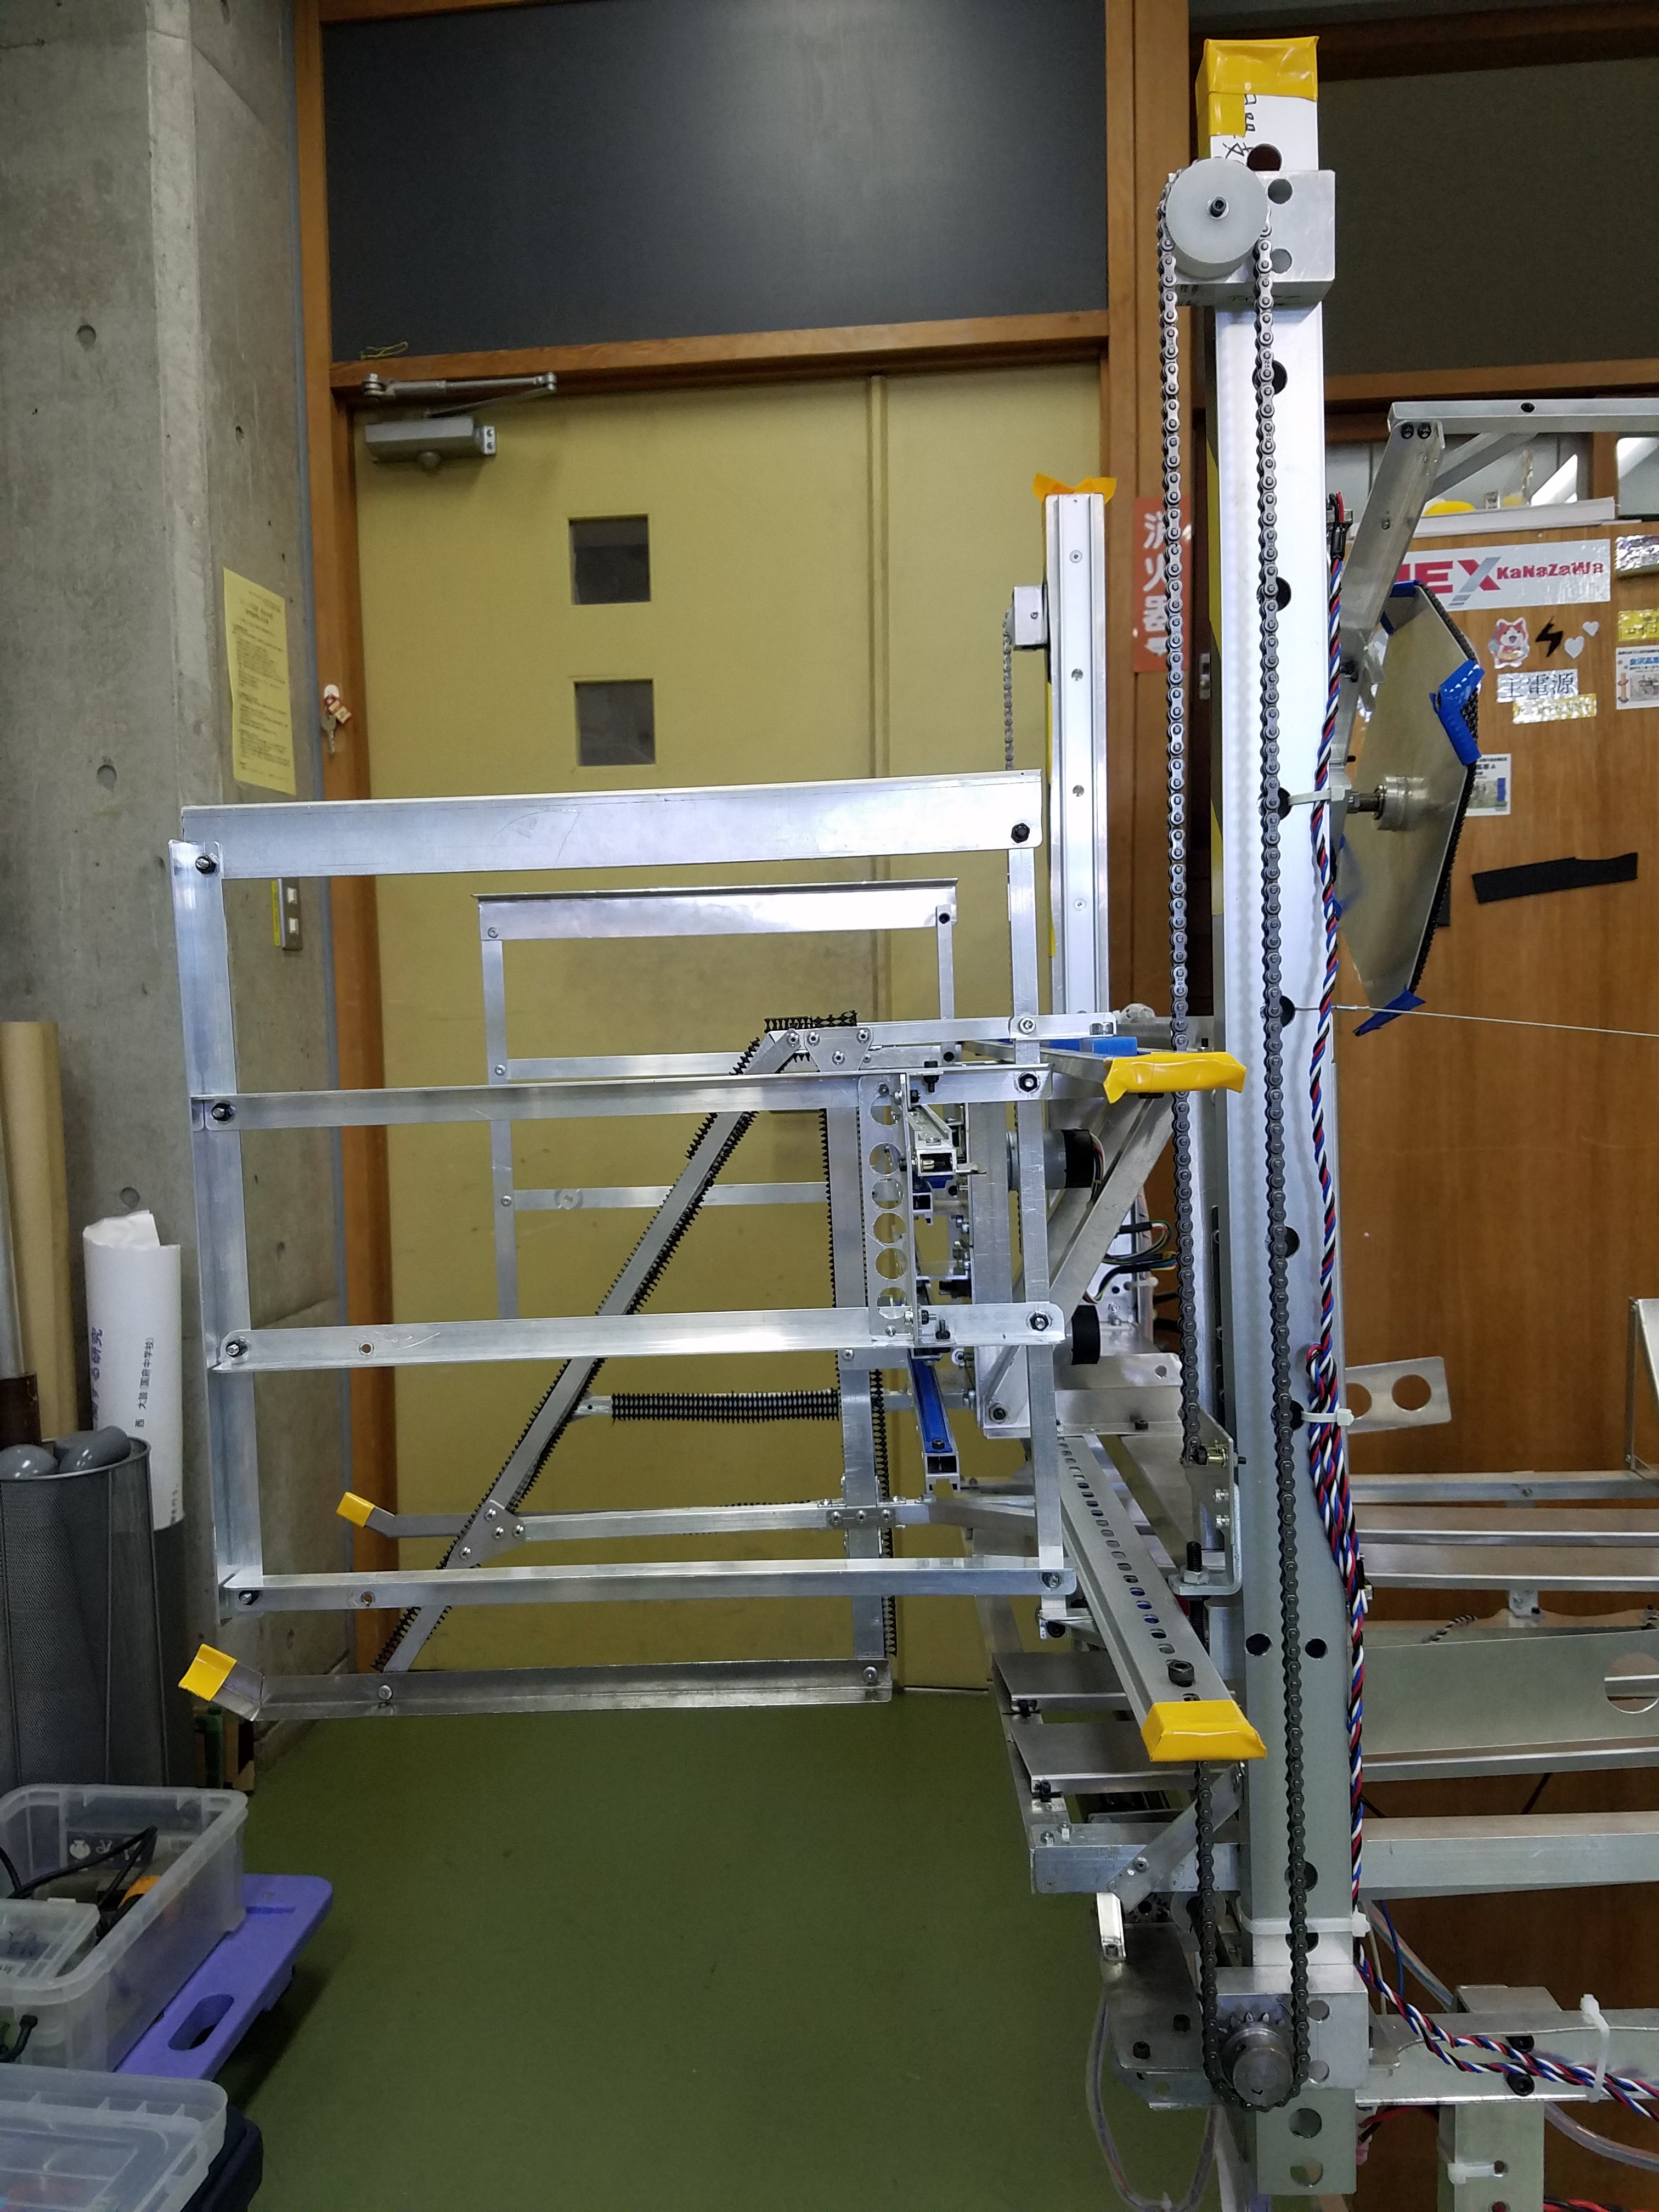
\includegraphics[width=80mm]{img/lift.jpg}
    \end{center}
  \caption{積み込みロボットのリフト}
 \label{fig:lift}
\end{figure}

\section{回路構造}
リフトに関わるロボットのシステムブロック線図は図\ref{fig:roboblock}のようになっている.arduinoは図\ref{fig:arduino}にあるようなarduinoMegaを使用した.このarduinoはUSBホストシールド(図\ref{fig:USBhs})を介したBluetoothでの通信でコントローラの信号を受け取る.コントローラでの操作と上下リミットセンサの信号を受け取り,図\ref{fig:motordrive}のモータドライバに指示を送り,リフト駆動用のモータを制御している.モータドライバはarduinoから正転,逆転,PWM値を受け取り,モータに最大12[V]の電圧を印加する.

\begin{figure}[htbp]
  \begin{center}
    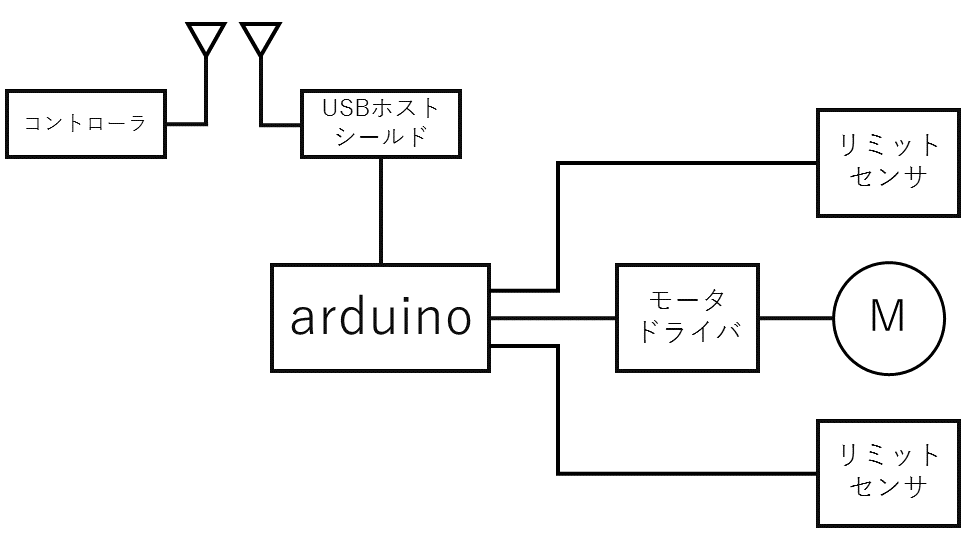
\includegraphics[width=120mm]{img/roboblock.png}
    \end{center}
  \caption{ロボットのシステムブロック線図}
 \label{fig:roboblock}
\end{figure}

\begin{figure}[htbp]
  \begin{center}
    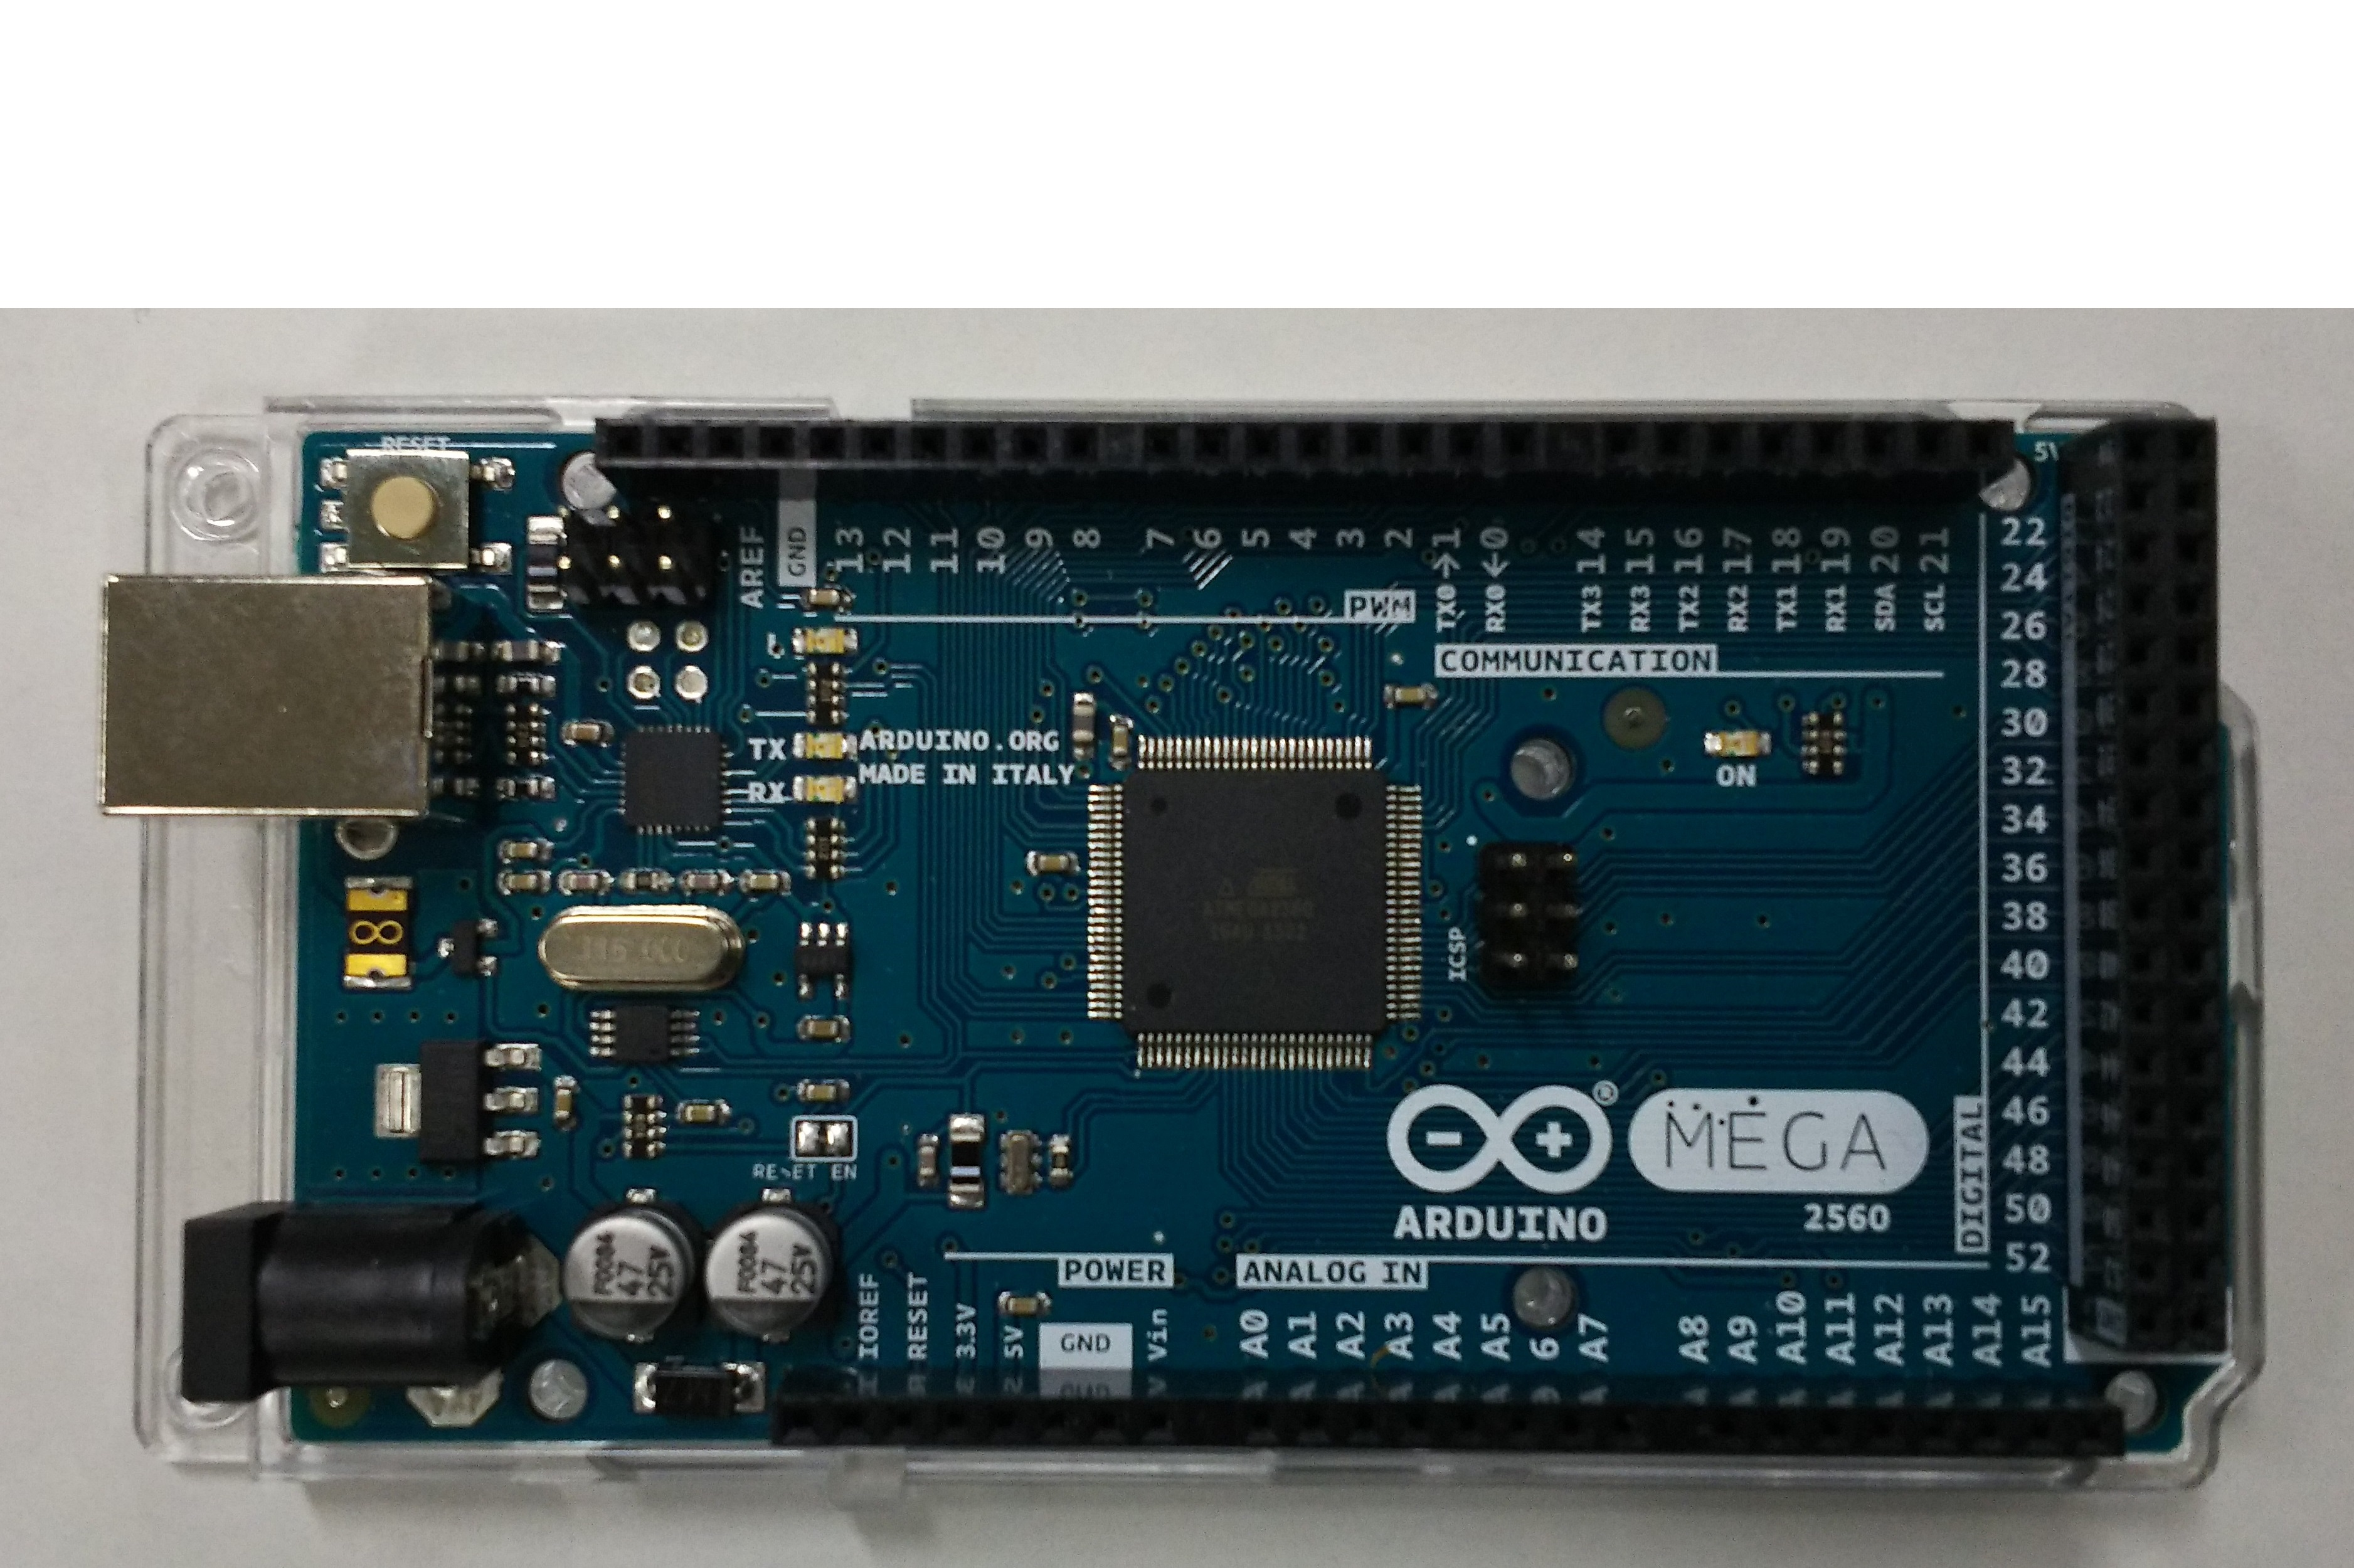
\includegraphics[width=100mm]{img/arduinoMega.JPG}
    \end{center}
  \caption{arduino Mega}
 \label{fig:arduino}
\end{figure}

\begin{figure}[htbp]
  \begin{center}
    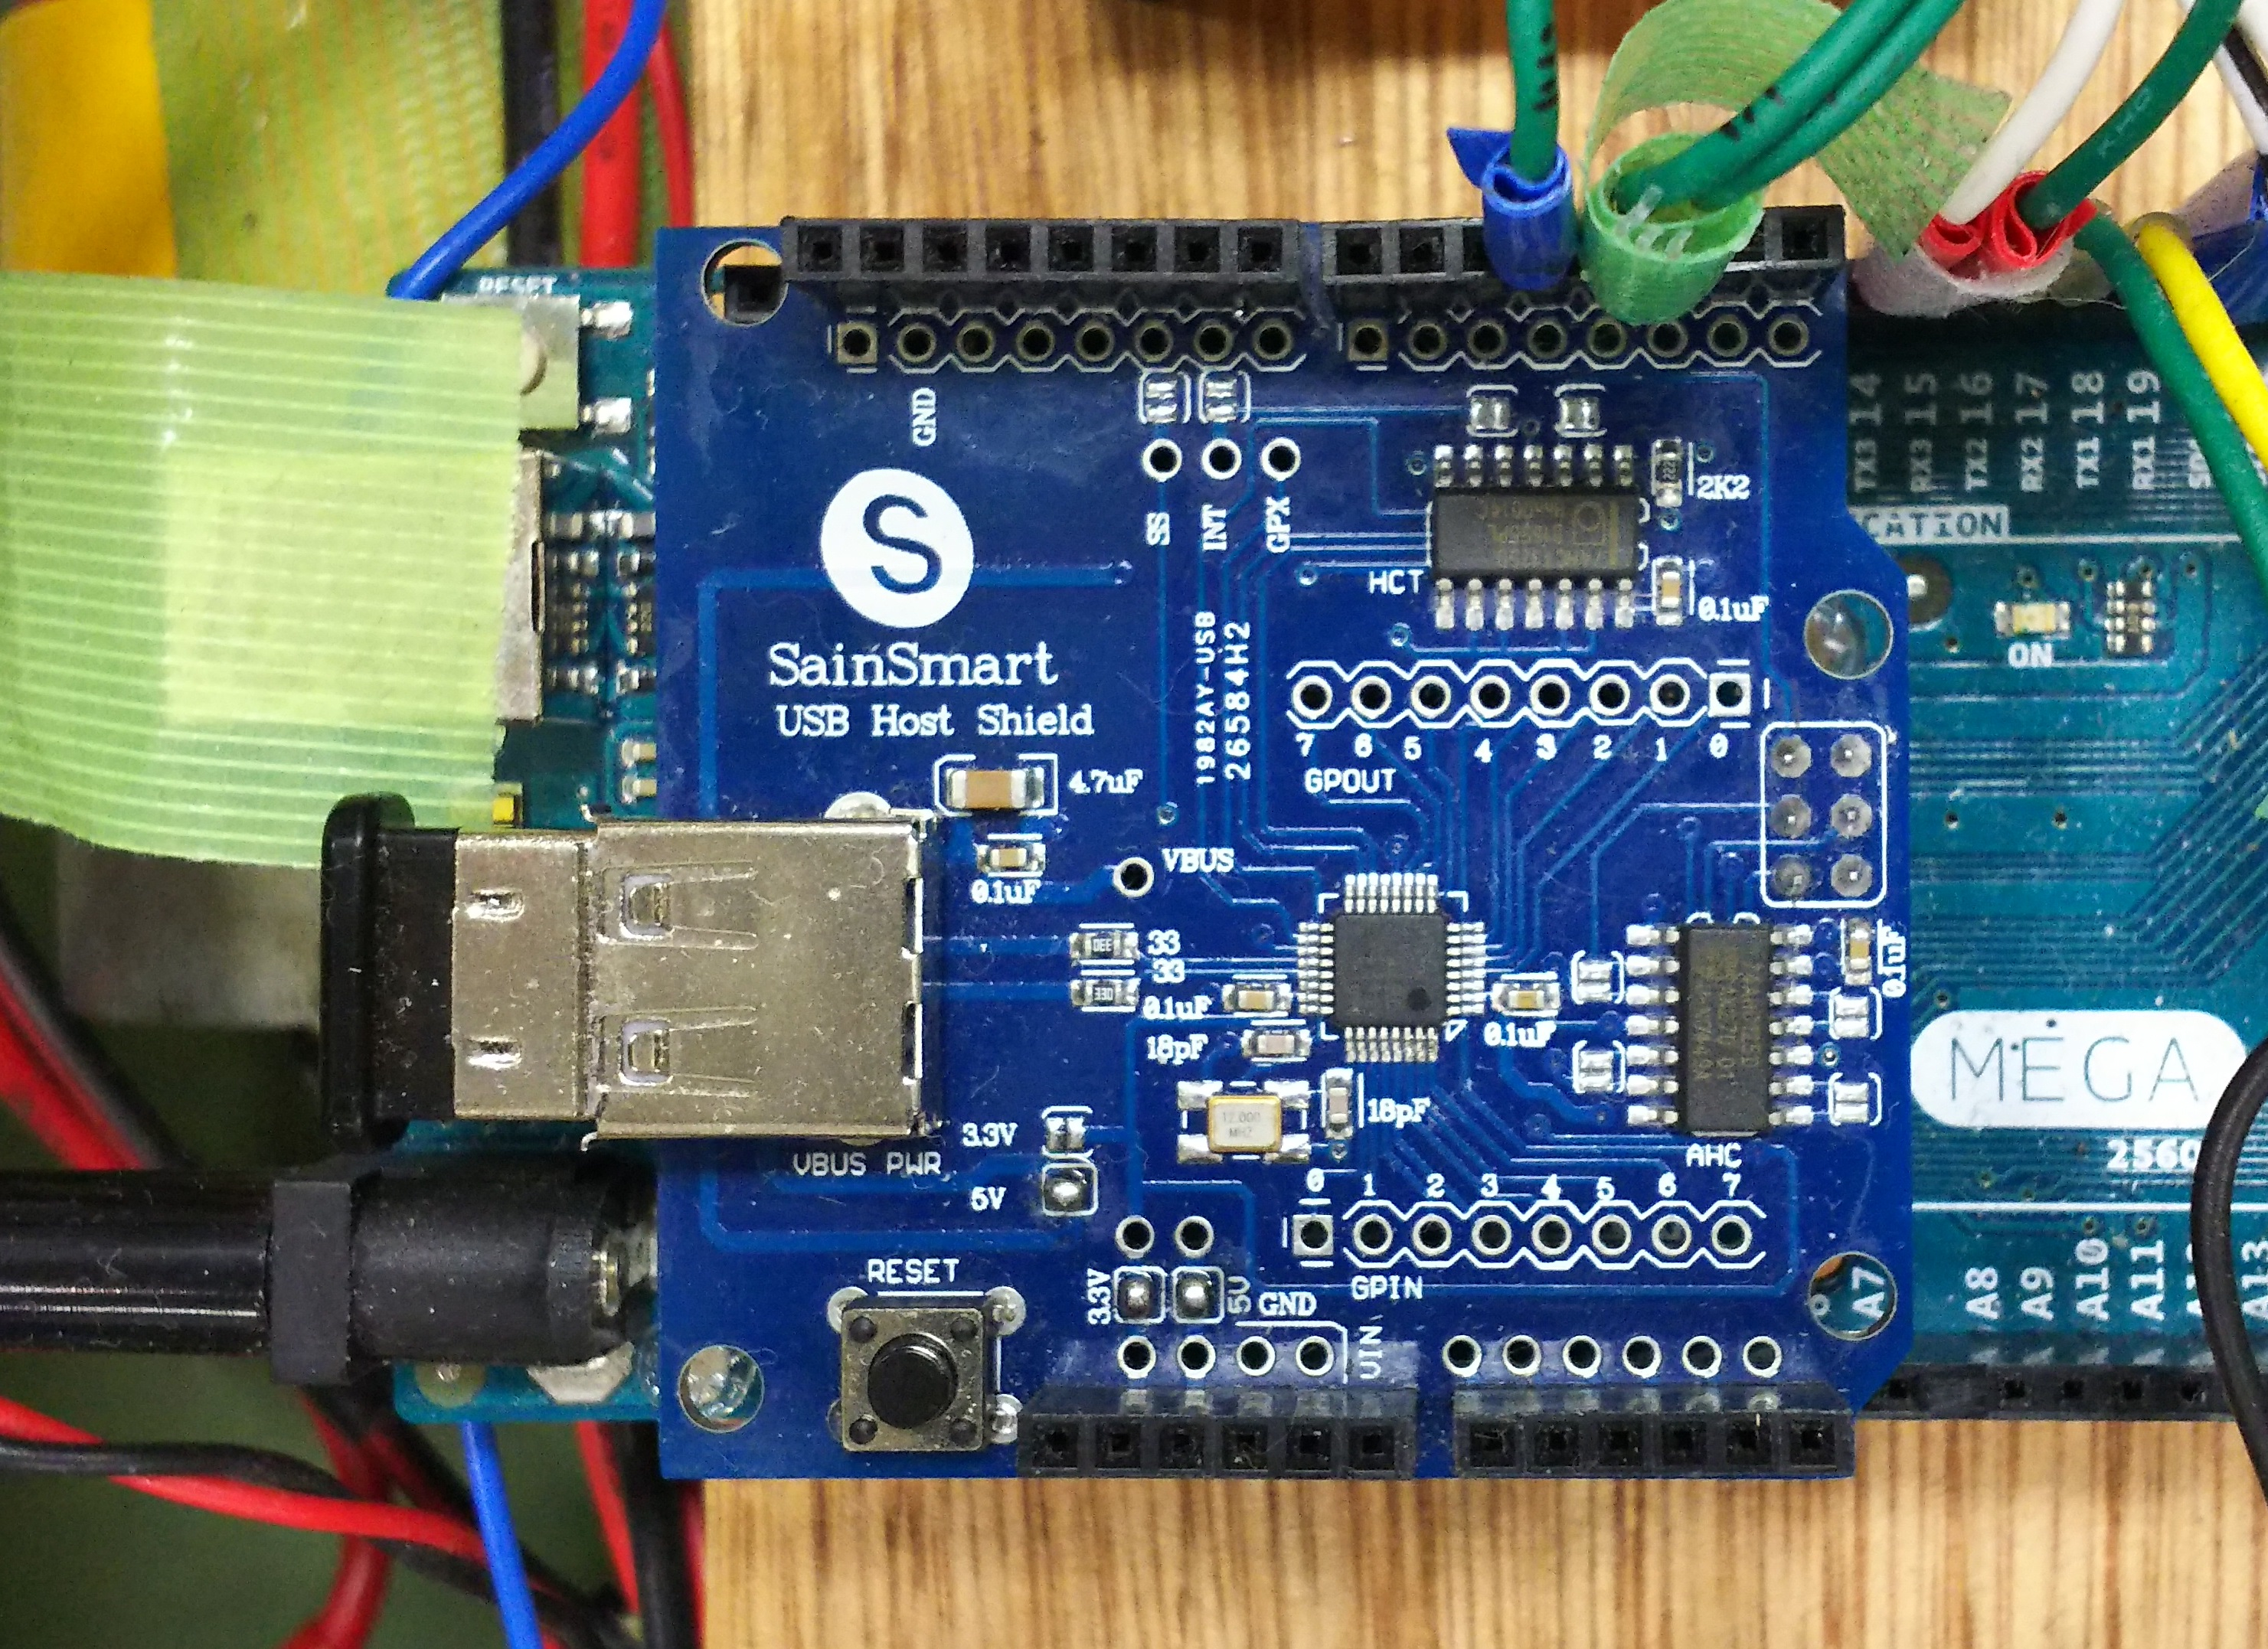
\includegraphics[width=100mm]{img/USBhs.JPG}
    \end{center}
  \caption{USBホストシールド}
 \label{fig:USBhs}
\end{figure}

\begin{figure}[!htbp]
  \begin{center}
    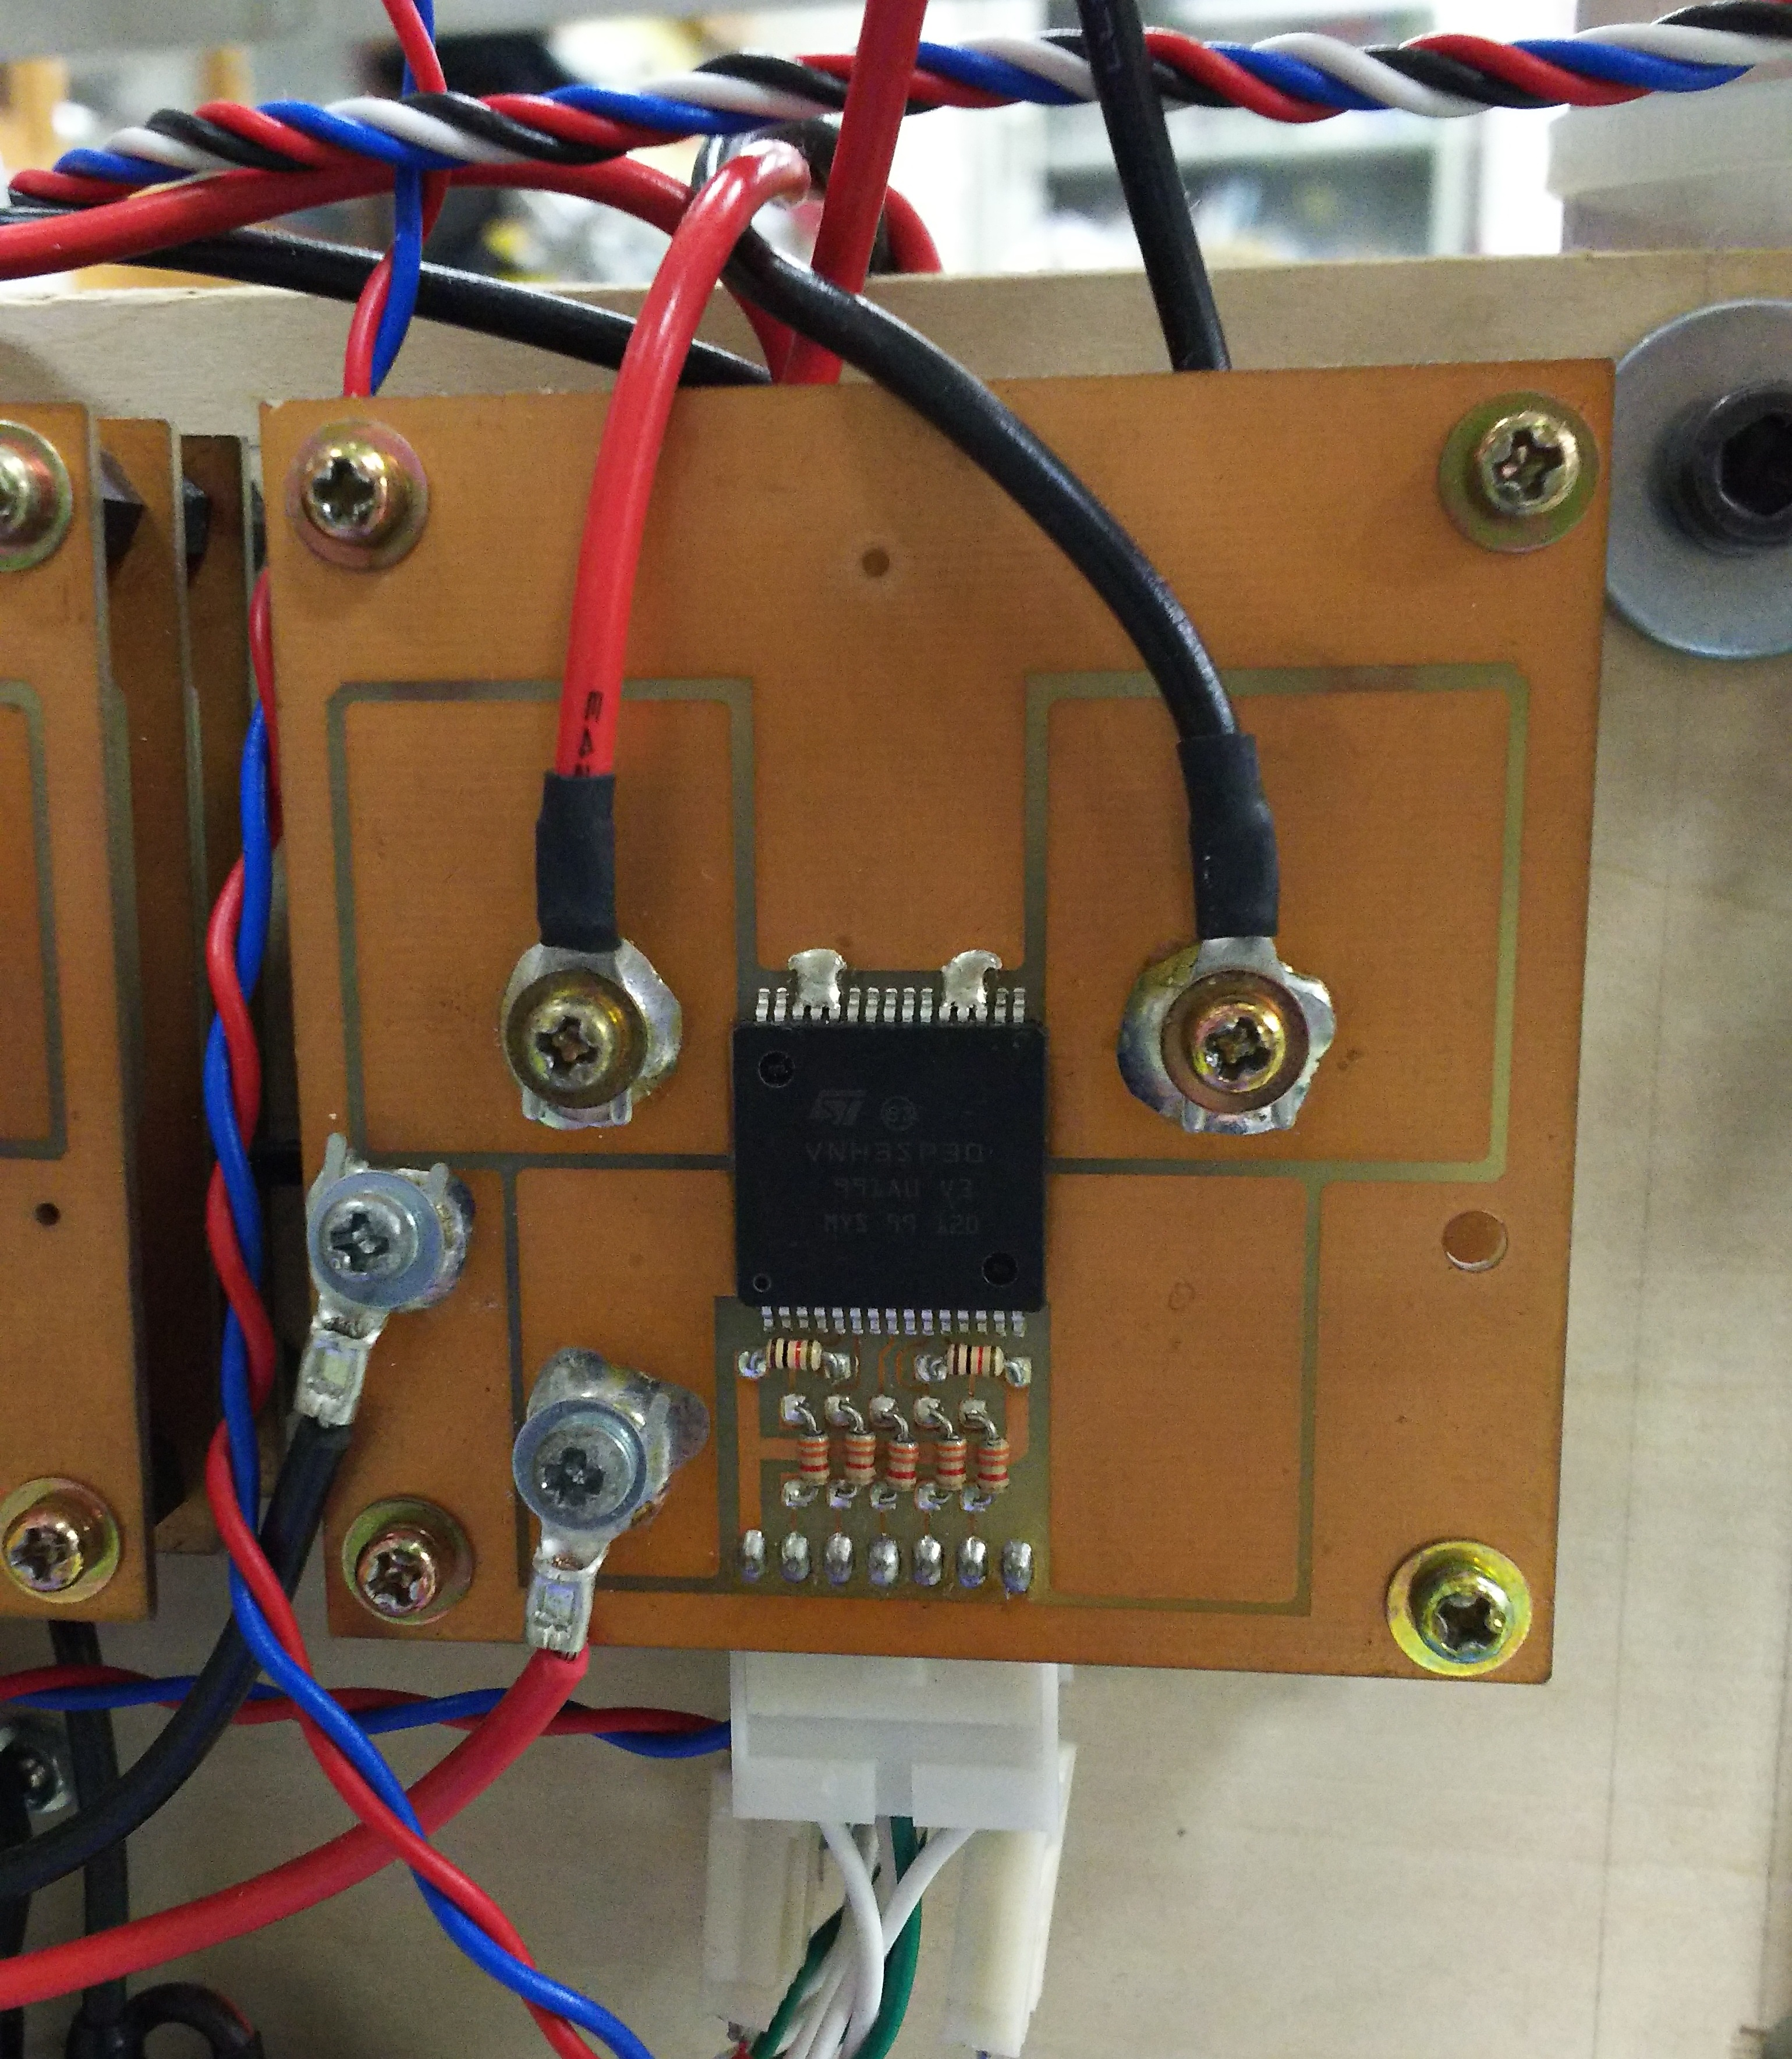
\includegraphics[width=90mm]{img/motordrive.JPG}
    \end{center}
  \caption{モータドライバ}
 \label{fig:motordrive}
\end{figure}

\section{使用部品}
使用した部品の詳細を以下の表\ref{tab:parts}に示す.

\begin{table}[!htb]
 \begin{center}
  \caption{搭載部品の型番とメーカ}
  \begin{tabular}[htbp]{|c|c|c|}
   \hline
   製品名&型番&メーカ \\
   \hline
   arduino&ArduinoMega&Arduino SRL\\
   \hline
   USBホストシールド&BOO6J4GOOO&サインスマート\\
   \hline
   DCモータ&組み合わせモータ323726&マクソン\\
   \hline
   コントローラ&DUALSHOCK3&ソニー\\
   \hline
   モータドライバ&-&夢考房\\
   \hline
   リミットセンサ&CNZ1023&パナソニック\\
   \hline
  \end{tabular}
  \label{tab:parts}
 \end{center}
\end{table}